\subsubsection{Technologien und Modelle}
\lfoot{Autor: Daniel Melichar}

Die Technologien und Konzepte der Web-Applikation sollen den benötigten Aufwand bei Weiterentwicklung der Applikation, sowie beim Hinzufügen von neuen Features, möglichst reduzieren. Grundsätzlich besteht jegliche Website (bei Web2.0 \cite{MELD.CH3-web-app.web2}) aus den folgenden Technologien.

\begin{description}
\item[HTML Markup \newline] \label{html} definiert den Inhalt eines Dokuments und gibt eine Struktur vor mittels dem Einsatz von Sektionen, Überschriften, Paragraphe, Listen, Menüs, und Formulare \cite{MELD.CH3-web-app.html}.

Eine konsequente, saubere, und ersichtliche Struktur ist wichtig, da durch den Einsatz von Ankern \textit{(engl.: Hooks)} die weitere Verarbeitung durch CSS und JavaScript passiert. Die Struktur hat auch eine große Wirkung auf die Flexibilität und zuverlässige Bereitstellung der Website.

Durch die Verwendung von Templates und Standards in einem Projekt ist es einfacher, gewisse Teile einer Web Applikation mehrmals zu verwenden, ohne die selbe Arbeit nochmals zu tätigen (siehe Seite \pageref{subsec:jsframeworks}).

\item[Cascading Style Sheets\newline] oder CSS, ist jener Teil einer Applikation, in welcher die visuelle Repräsentation und Design Regeln beschrieben werden. Ein gut geschriebenes CSS verwendet das kaskadenförmige Prinzip der Sprache – generelle Regeln werden zuerst inkludiert und danach die überschreibenden für spezifische Instanzen \cite{MELD.CH3-web-app.css}.

Es ist sehr einfach, mit CSS inkonsistenten und unnötigen Code zu schreiben, welcher dann so fragil ist, so dass es auf der Webseite immer wieder kleine Unterschiede gibt. Aufgrund dessen sollte CSS immer \cite{MELD.CH3-web-app.css2}
\begin{enumerate}
\item einfach zu verwalten sein
\item klar ersichtliche Patterns haben
\item das Einfügen von neuen Stilvorgaben ermöglichen
\item nicht verwendete Stilvorgaben weglassen
\item möglichst viele Geräte und Browser Versionen unterstützen
\item Standardwerte setzen
\item Unterscheiden zwischen globalen und spezifischen Styles
\end{enumerate}

Bevor es an das eigentliche Erstellen von Code geht sollte man vorab immer das vorgegebene Design überprüfen, ein technisches Konzept erstellen und hierbei vor allem auf logische Verknüpfungen im Code achten. Das bedeutet konkret, dass die Styles des Kunden (bzw. deren Corporate Identity) in die Webseite eingeplant, die Basis der Typographie der Webseite erstellt, und Styles für die komplette Webseite bzw für spezifische Sektionen erstellt werden müssen.

\textbf{Tools und Frameworks\newline}
In manchen Fällen ist die Verwendung von CSS-Libaries sehr hilfreich. Diese sollten aber aus einem guten Grund gewählt werden. Auch hier gibt es wiederum viele Arten von Tools, die Verwendet werden können \cite{MELD.CH3-web-app.css3}. Einige können als eigene, bessere Sprachen angesehen werden, welche sich dann einfach zu CSS konvertieren, Andere reduzieren den bereits vorhanden Code auf das Minimum.

Vorgefertigte UI Komponenten oder CSS Frameworks, können ebenfalls sehr hilfreich sein \cite{MELD.CH3-web-app.css3}, aber auch hier gilt: nur verwenden, wenn wirklich notwendig. Wiederum gibt es verschiedene Kategorien von Frameworks die für verschiedenstes verwendet werden können: UI Komponenten oder Widget libraries (z.B. Bootstrap, jQuery UI), Grid Systems, Typographie Anpassungen, Normalisierung von Code.


\item[JavaScript\newline]
beschreibt zusätzliche Verhaltensweisen, Features und Funktionalität, welche normalerweise nicht von Web Browsern durch den Einsatz von CSS und HTML unterstützt werden. In den letzten Jahren hat JavaScript einen enormen Boom erhalten \cite{MELD.CH3-web-app.js2}. Dies ist aufgrund der immer größeren Anzahl an Features, schnelleren Browsern und Server Laufzeitumgebungen wie Node.js, welche stetig auf den letzten Standpunkt gebracht werden \cite{MELD.CH3-web-app.js1}. 

Es gibt mittlerweile für beinahe jede Komponente einer Website, eine JavaScript Library oder Framework \cite{MELD.CH3-web-app.js3}. Man sollte dennoch nur dann JavaScript verwenden, wenn keine andere Möglichkeit existiert.  Sollte der Fall eintreten, und es wirklich keine native Funktion durch CSS/HTML gibt, muss die JavaScript Komponente auf Performance getestet werden. Auch hier gilt es dann möglichst schnellen, effizienten und performanten, wiederverwendbaren Code zu generieren. 

Für die Auswahl von Third Party Projekten oder Code sollten folgende Punkte bei der Überlegung eingebunden werden:
\begin{enumerate}
\item Technische Requirements 
\item Qualität und Reife
\item Zukünftiger Support
\item Entwickler und Community des Projekts / Code
\item Testung auf verschiedensten Plattformen und Geräten
\end{enumerate}

Viel zu oft vergessen Entwickler von Web-Applikationen das Gesamtkonzept und fokussieren sich nur auf einen geringen Teil - eine Ansammlung an Plugins ist keine gute Lösung. Deshalb sollte JavaScript hauptsächlich für die folgenden Komponenten und/oder Eigenschaften verwendet werden:
\begin{enumerate}
\item Document Object Model (DOM) Manipulation
\item Ajax Validation
\item Query String Konverter
\item Tests für globale Konditionen (z.B. Bildschirmgröße, Feature Support)
\item UI Controls
\item Datum Selektion
\end{enumerate}
\end{description}

\textbf{Verwendung und Anwendung\newline}
\lfoot{Autor: Hüseyin Bozkurt}
\label{subsec:jsframeworks}
Für die konkrete Umsetzung einer Web-Applikation wird in den meisten Fällen ein Framework gewählt, welches die Möglichkeit bietet, alle Eigenschaften einer Webseite zu erstellen (HTML für die Struktur, CSS für das Aussehen, JavaScript für Funktionalität). Mittels dem MVC-Konzept \cite{MELD.CH3-web-app.js4} wird dem Entwickler des Systems die Arbeit leichter gemacht.

\begin{table}[!htb]
\centering
\resizebox{\columnwidth}{!}{%
\begin{tabular}{ll}
\hline
\multicolumn{2}{|c|}{\textbf{Angular 2.0}}                                                                                                                                                                                   \\ \hline
\multicolumn{1}{|c|}{\textbf{Stärken}}                                                                                                                                 & \multicolumn{1}{c|}{\textbf{Schwächen}}             \\ \hline
\multicolumn{1}{|l|}{Performance}                                                                                                                                      & \multicolumn{1}{l|}{Dokumentation ist eher schwach} \\ \hline
\multicolumn{1}{|l|}{Rendering am Server}                                                                                                                              & \multicolumn{1}{l|}{}                               \\ \hline
\multicolumn{1}{|l|}{Native GUI}                                                                                                                                       & \multicolumn{1}{l|}{}                               \\ \hline
\multicolumn{1}{|l|}{\begin{tabular}[c]{@{}l@{}}Herangehensweise eines Frameworks \\ (spezifische Funktionen von Angular \\ können einfach entfernt werden)\end{tabular}} & \multicolumn{1}{l|}{}                               \\ \hline
\multicolumn{1}{|l|}{ES2015 Standard includiert}                                                                                                                       & \multicolumn{1}{l|}{}                               \\ \hline
\multicolumn{1}{|l|}{Große Community}                                                                                                                                  & \multicolumn{1}{l|}{}                               \\ \hline
\multicolumn{1}{|l|}{Einfache testung} & \\ \hline                                                           
\end{tabular}
}
\caption{Angular 2.0 - \url{https://angular.io/}}
\end{table}

\textbf{Angular 2.0} ist ein Framework, welches dabei helfen soll, Client Applikationen in HTML und JavaScript zu entwickeln. Das Framework an sich besteht aus mehreren kooperierenden Libaries. Für die Erstellung einer Angular Applikation müssen so gennante HTML \textit{templates} im Angular-Stil erstellt werden, einige \textit{component} Klassen welche die templates managen dazu einbinden, und die Logik hinter der Applikation in so gennanten \textit{services}, beschreiben \cite{MELD.CH3-web-app.angular}. Für eine Beschreibung zur Architektur, siehe Abbildung \ref{fig:angulararch}.

\clearpage

\begin{table}[!htb]
\centering
\resizebox{\columnwidth}{!}{%
\begin{tabular}{ll}
\hline
\multicolumn{2}{|c|}{\textbf{Ember 2.0}}                                                                                                                                                                                                                                            \\ \hline
\multicolumn{1}{|c|}{\textbf{Stärken}}                                                                                                                                    & \multicolumn{1}{c|}{\textbf{Schwächen}}                                                                 \\ \hline
\multicolumn{1}{|l|}{Performance}                                                                                                                                         & \multicolumn{1}{l|}{\begin{tabular}[c]{@{}l@{}}Schwirige Anwendung in speziellen\\ Fällen\end{tabular}} \\ \hline
\multicolumn{1}{|l|}{Rendering am Server}                                                                                                                                 & \multicolumn{1}{l|}{Kleinere Community}                                                                 \\ \hline
\multicolumn{1}{|l|}{Native GUI}                                                                                                                                          & \multicolumn{1}{l|}{}                                                                                   \\ \hline
\multicolumn{1}{|l|}{\begin{tabular}[c]{@{}l@{}}Herangehensweise eines Frameworks \\ (spezifische Funktionen von Angular \\ können einfach entfernt werden)\end{tabular}} & \multicolumn{1}{l|}{}                                                                                   \\ \hline
\multicolumn{1}{|l|}{Dokumentation}                                                                                                                                       & \multicolumn{1}{l|}{}                                                                                   \\ \hline
\multicolumn{1}{|l|}{CLI Tools} & \\ \hline                                                                   
\end{tabular}
}
\caption{Ember 2.0 \url{http://emberjs.com/}}
\end{table}

\textbf{Ember.js 2.0} ähnelt sehr stark dem Angulars Architektur Konzept. Der Grund wieso wir Ember nicht verwenden basiert auf der simplen, etwas schöneren API von Angular. Fakt ist, dass Angular keine weiteren Dependencies hat (Ember.js verwendet jQuery und Handlebars) und dass Angular eine viel geringere Filegröße hat\cite{MELD.CH3-web-app.ember}. Für eine Graphik der Ember Architektur, siehe Abb. \ref{fig:emberarch}.

\begin{table}[!htb]
\centering
\resizebox{\columnwidth}{!}{%
\begin{tabular}{ll}
\hline
\multicolumn{2}{|c|}{\textbf{React 1.0}}                                                                                                                                                                                                                                                             \\ \hline
\multicolumn{1}{|c|}{\textbf{Stärken}}                                                                                                                                    & \multicolumn{1}{c|}{\textbf{Schwächen}}                                                                                  \\ \hline
\multicolumn{1}{|l|}{Performance}                                                                                                                                         & \multicolumn{1}{l|}{\begin{tabular}[c]{@{}l@{}}Andere Architektur als bei gängigen\\ Frameworks / Libaries\end{tabular}} \\ \hline
\multicolumn{1}{|l|}{Rendering am Server}                                                                                                                                 & \multicolumn{1}{l|}{Unnötig hinzugefügte Features}                                                                       \\ \hline
\multicolumn{1}{|l|}{Native GUI}                                                                                                                                          & \multicolumn{1}{l|}{}                                                                                                    \\ \hline
\multicolumn{1}{|l|}{\begin{tabular}[c]{@{}l@{}}Herangehensweise eines Frameworks \\ (spezifische Funktionen von Angular \\ können einfach entfernt werden)\end{tabular}} & \multicolumn{1}{l|}{}                                                                                                    \\ \hline
\multicolumn{1}{|l|}{Einfach anzuwenden}                                                                                                                                  & \multicolumn{1}{l|}{}                                                                                                    \\ \hline
\multicolumn{1}{|l|}{ES2015 Standard includiert} & \\ \hline                                                                   
\end{tabular}
}
\caption{React 1.0 \url{https://facebook.github.io/react/}}
\end{table}

Das von Facebook entwickelte \textbf{React.js} ist ein eher spezielles Framework, oftmals wird gesagt, dass React.js das \textbf{V} im MVC-Konzept (Model-View-Control) da bietet. Aufgrund dessen ist die Filegröße des Frameworks um einiges kleiner als bei den anderen beiden, bietet aber dennoch viele der Basis Features an \cite{MELD.CH3-web-app.react}. Leider bietet React nicht alles an, was für unsere Applikation benötigt wird, daher ging es rasch aus der ängeren Auswahl raus.Für eine Graphik der React Architektur, siehe Abb. \ref{fig:reactarch}.

\begin{figure}[!tbp]
 	\centering
 	\begin{minipage}[b]{0.8\textwidth}
 		\centering
 		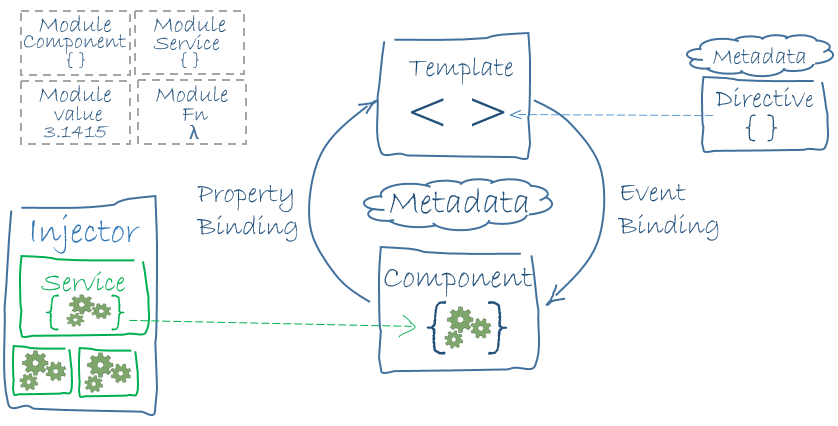
\includegraphics[width=0.8\textwidth]{images/angular}
		\caption{Angular Architektur \cite{MELD.CH3-web-app.angular}}
		\label{fig:angulararch}
 	\end{minipage}
 	\hfill
 	\begin{minipage}[b]{0.8\textwidth}
 		\centering
 		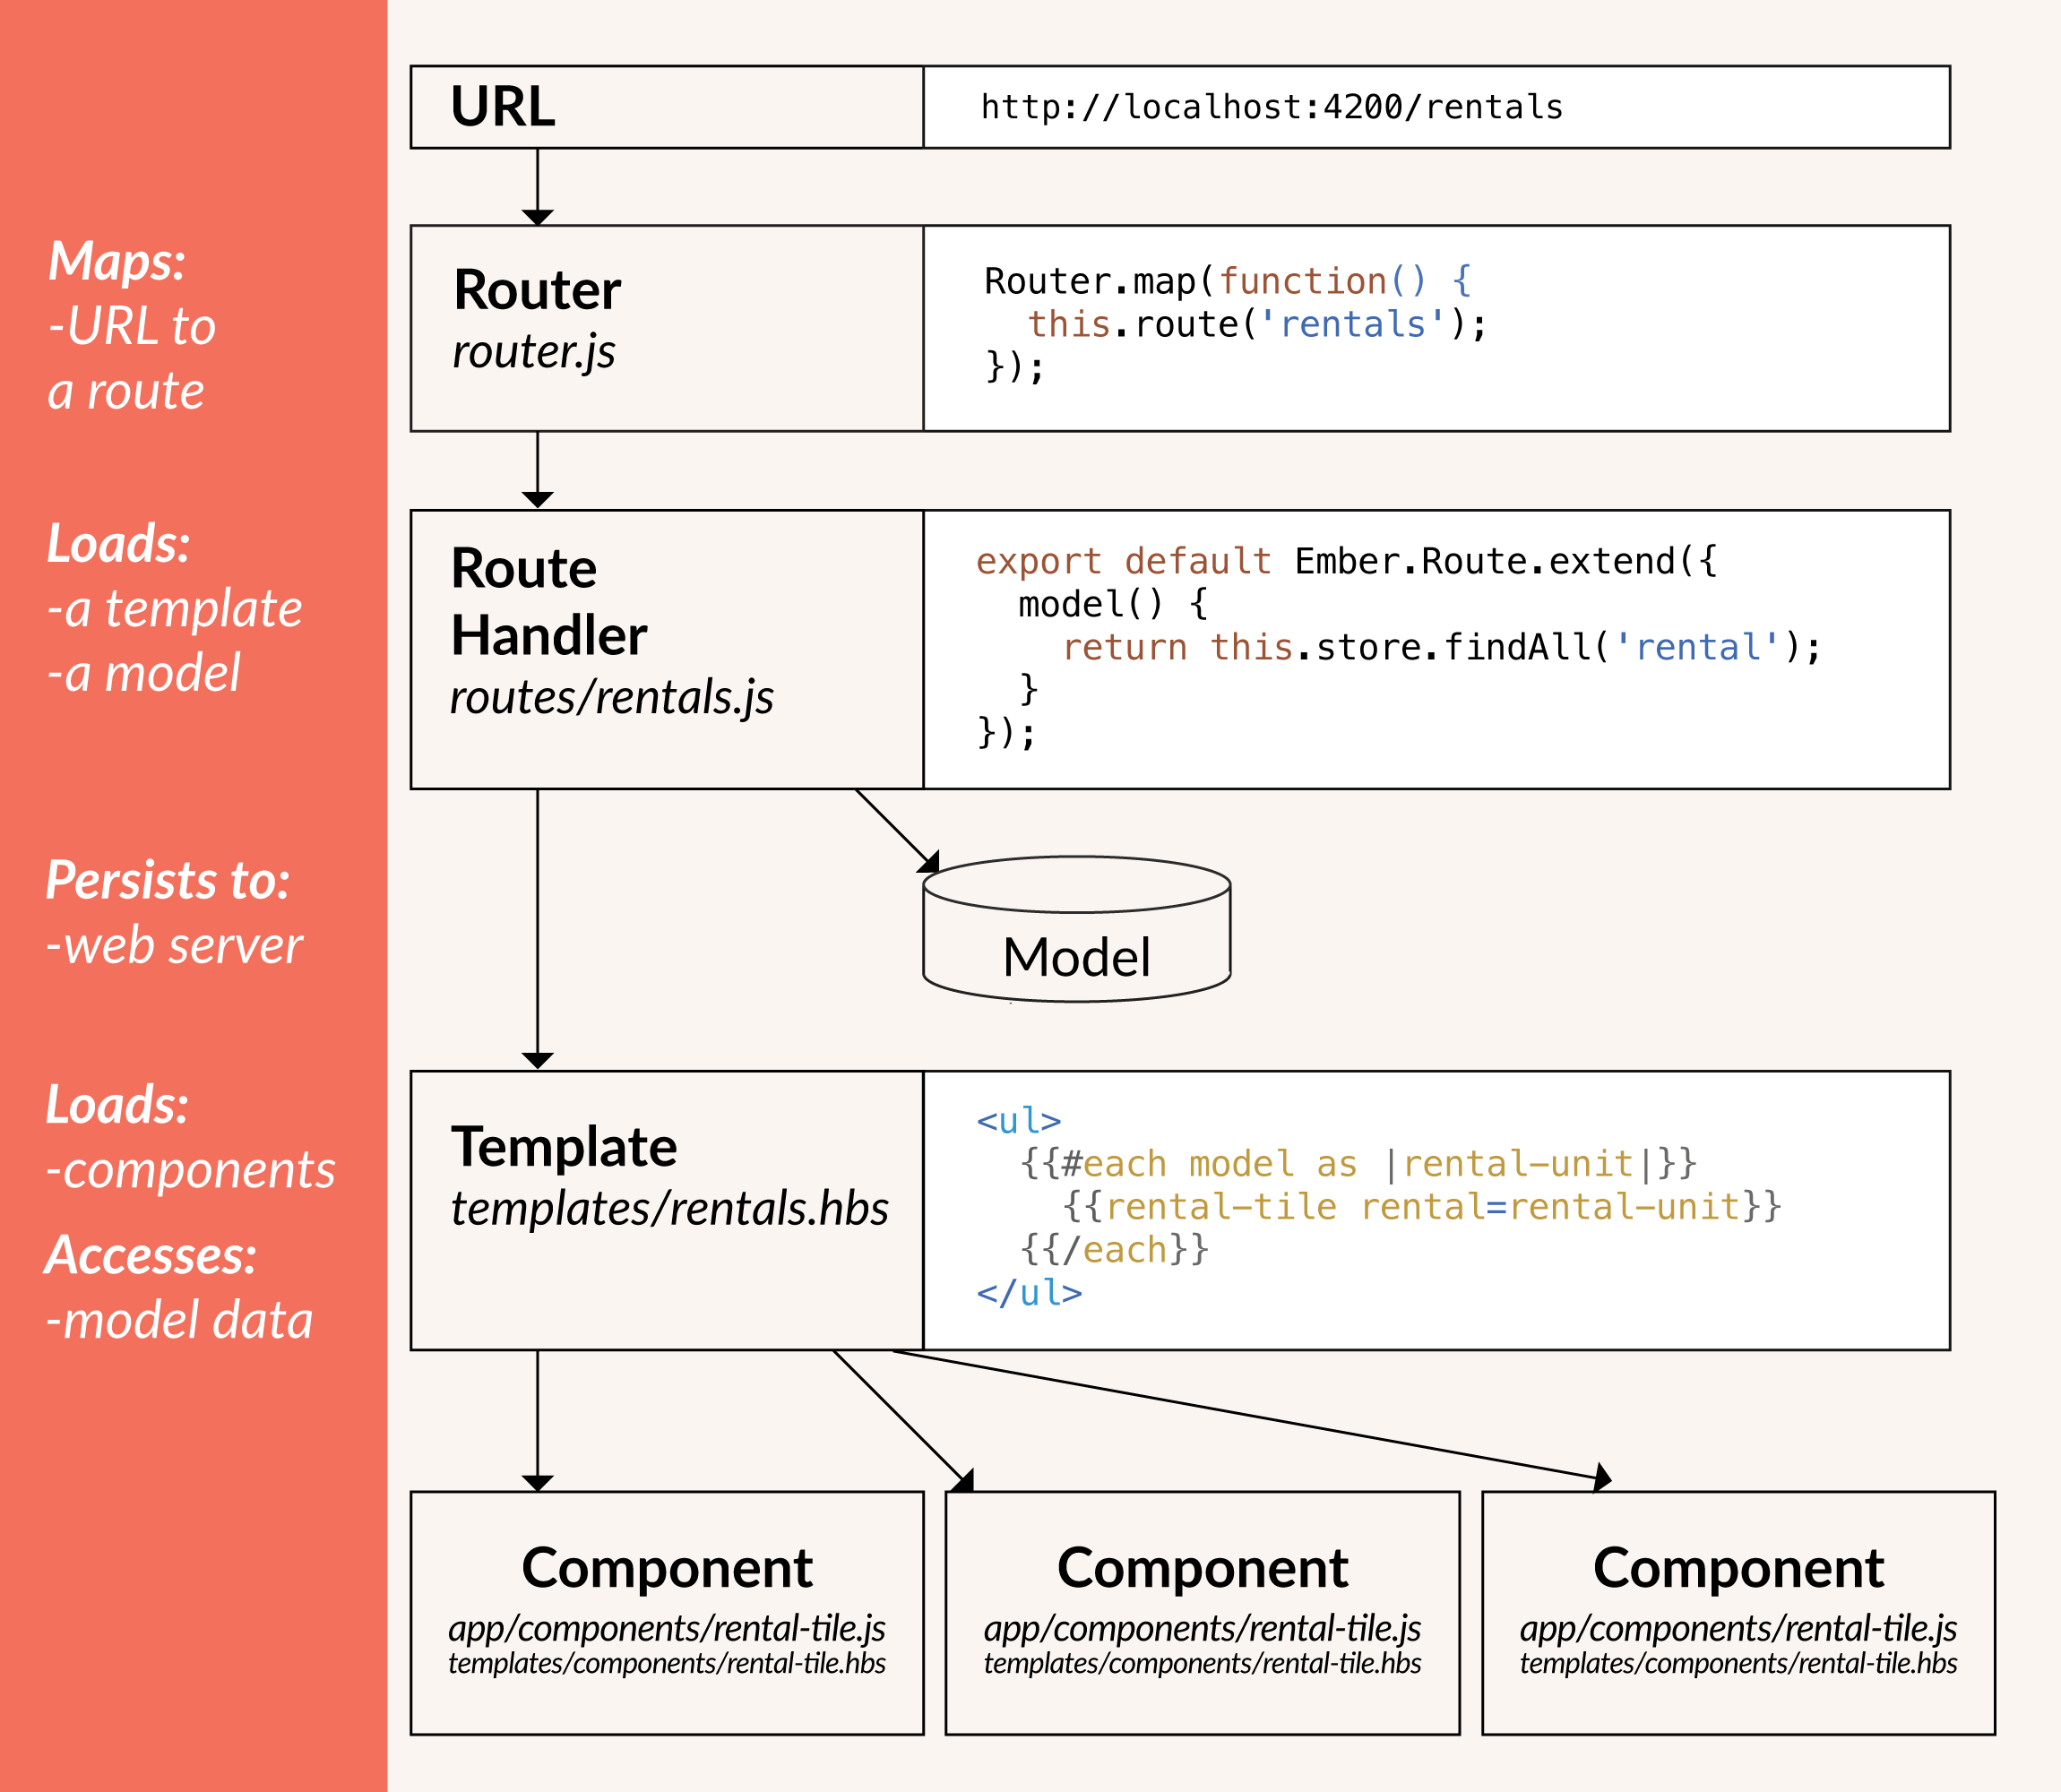
\includegraphics[width=0.8\textwidth]{images/ember}
		\caption{Ember Architektur \cite{MELD.CH3-web-app.ember}}
		\label{fig:emberarch}
 	\end{minipage}
 	\hfill
 	\begin{minipage}[b]{0.7\textwidth}
 		\centering
		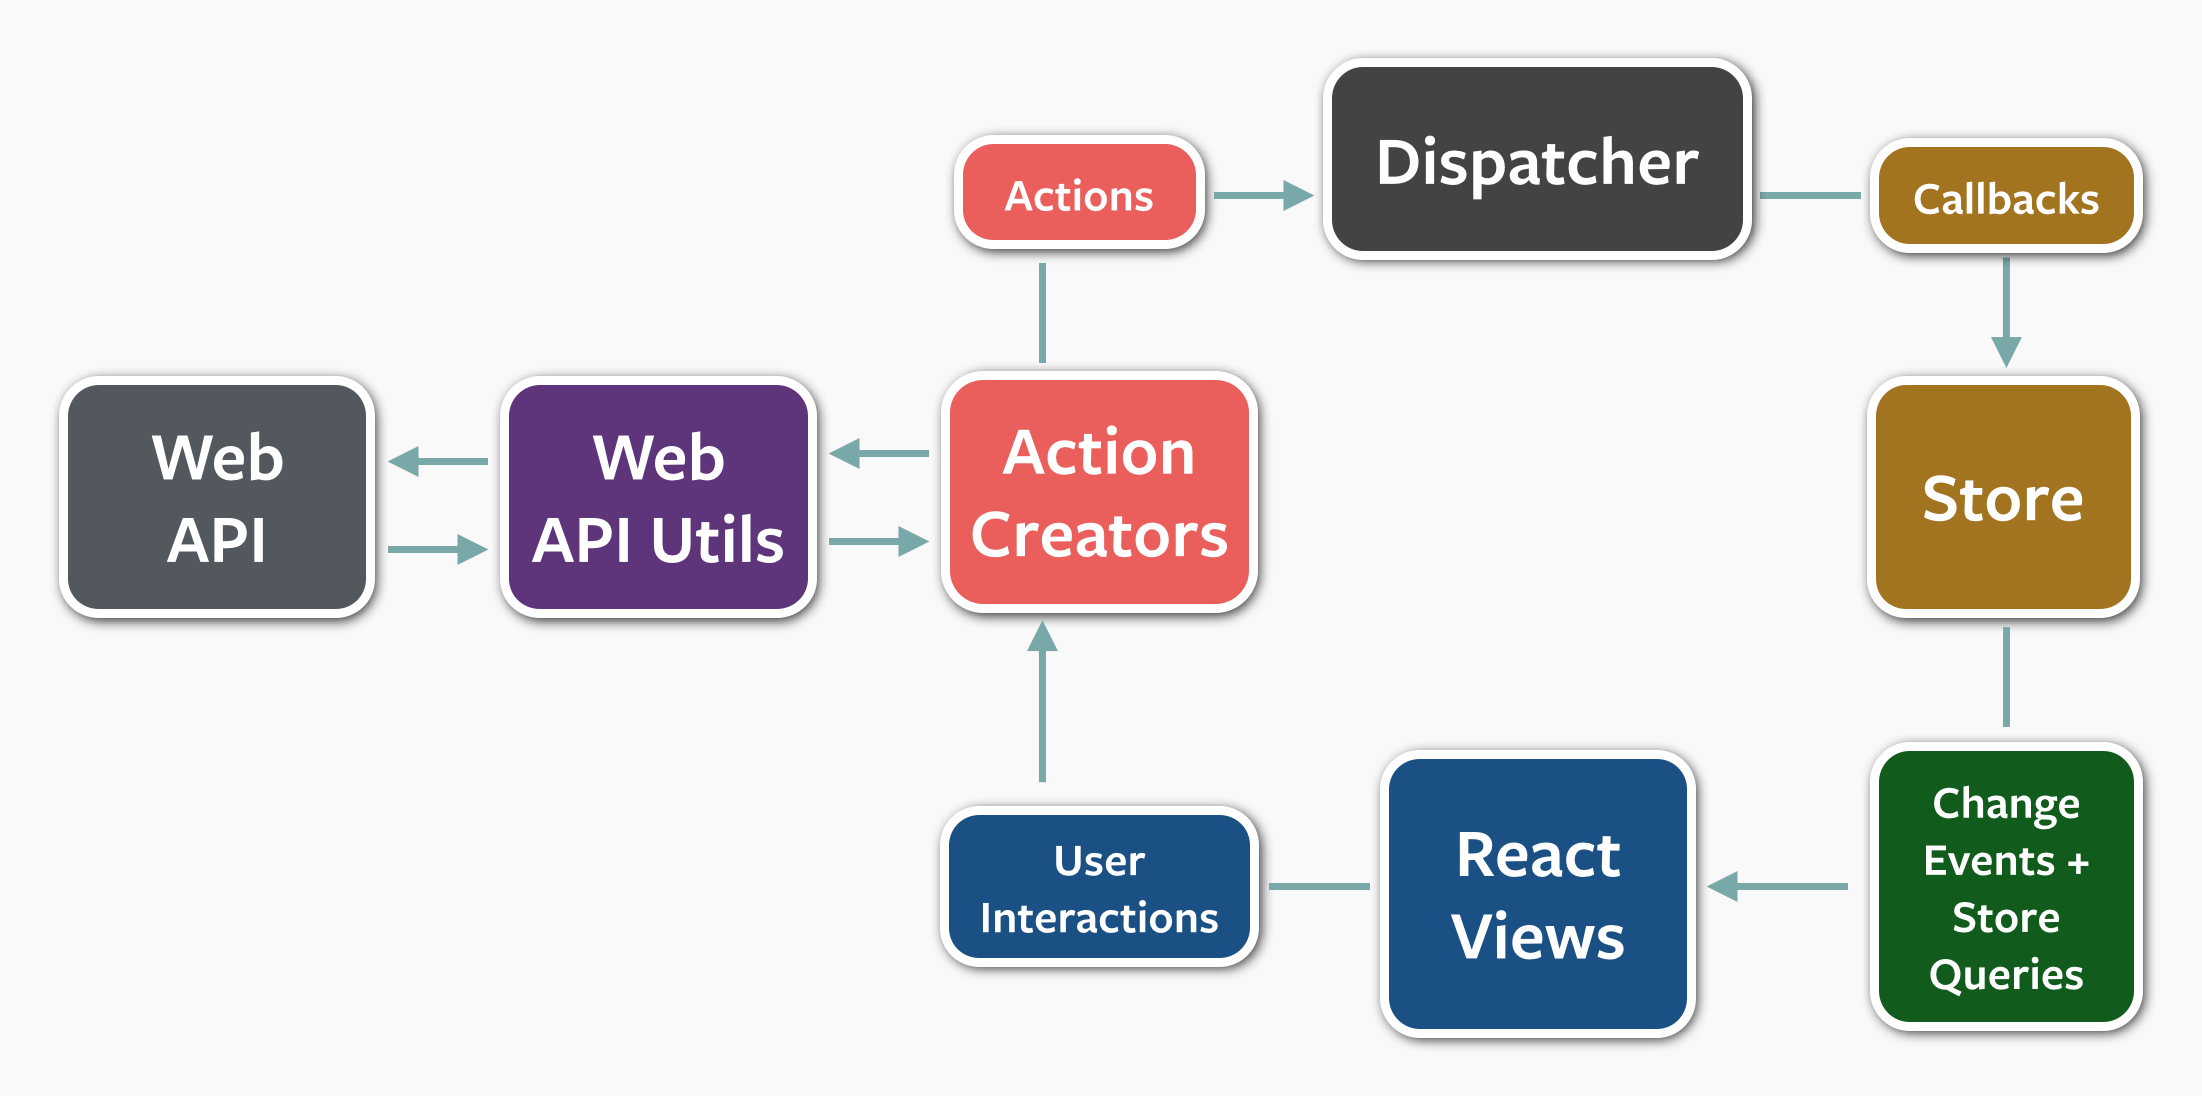
\includegraphics[width=0.7\textwidth]{images/react}
		\caption{React Architektur \cite{MELD.CH3-web-app.react}}
		\label{fig:reactarch}
 	\end{minipage}
\end{figure}

